\subsection{The concretisation function}
\label{sec:app_concret}

Let $s = (E,\seq,\cover,\prec,\dashv,\labl)$ be a linear extension of an augmented poset.
In the algorithm proposed on~\autoref{sec:concret} we change~\autoref{eq:refine} so that instead of computing a new decoration for each new poset $s_2$ (\autoref{eq:dec}), we use the existing decoration $(s_1)^{\star}$ of $s_1$ and only refine the trace w.r.t. to the decorations for the new event $e$ added to the trace.

Also we change the interpretation of the refinement function $\mathtt{Ref}$: instead of a bijection between events and transitions in $\theta$, we use a bijection between events and transitions positions in $\theta$ (\autoref{eq:ith_trans}). The update of $\mathtt{Ref}_1$ to $\mathtt{Ref}_2$ is then straightforward.

\begin{align}
  &\mathsf{concretise}(s,s_1,\mathit{concretisations}_1) = \\
  &\quad\text{if }(E_s\setminus E_{s_1} = \emptyset)\text{ then return }\mathit{concretisations}_1\\
  &\quad e = \text{min}_{\sqsubset}(E_s\setminus E_{s_1})\\
  &\quad\mathit{concretisations}_2 = \emptyset \\
  &\quad\text{for each }(\theta_1,\mathtt{Ref}_1)\text{ in }\mathit{concretisations}_1\\
  &\quad\qquad s_2 = s\setminus\{s_1\cup\{e\}\}\\
  \label{eq:dec}
  &\quad\qquad\text{for each }(s_2)^{\star}\text{ in }\mathsf{decorate}(s_2)\\
  &\quad\qquad\qquad (s_1)^{\star} = \mathsf{decoration\_of\_trace}(\theta_1)\\
  &\quad\qquad\qquad \text{ if }s_2^{\star}\subseteq (s_1)^{\star}\text{ and }\mathsf{valid}(s_2^{\star})\text{ then }\\
  &\quad\qquad\qquad\qquad \mathit{spans} = \mathsf{decorations\_for\_last\_event}(s_2^{\star})\\
  \label{eq:refine}
  &\quad\qquad\qquad\qquad \mathit{\theta_2} = \mathsf{refine}(\theta_1,\mathtt{Ref}_1,\labl(e),\mathit{spans})\\
  &\quad\qquad\qquad\qquad \mathtt{Ref}_2 = \mathtt{Ref}_1\cup\{e\leftrightarrow\mathsf{length}(\theta_2)\}\\
  &\quad\qquad\qquad\qquad \mathit{concretisations}_2 = \mathit{concretisations}_2 \cup (\mathit{\theta_2},\mathtt{Ref}_2)\\
  &\quad\text{return }\mathit{concretisations}_2
\end{align}

%%%%%!!alternative : discover on the fly the decorations (let's call them discovered-deco) between the last transition in the trace $\theta$ and the new production $\labl(e)$. Then have to show that all decorations are preserved by the discovered-deco. A start is in the file \subsection{Refinement of graph rewriting rules}

\begin{definition}[Refinement of two rewriting rules using positive influence]
  \label{def:ref_pos_infl}
  Let $r_1:L_1\remb K_1 \lemb R_1$ and $r_2:L_2\remb K_2 \lemb R_2$ be two rules and let $s$ be a cospan such that $r_1\redl{+}_s r_2$. Define the refinement of $r_1$ and $r_2$ using $s$, $r_1\oplus_s r_2 = M_1\remb K\lemb M_2$ obtained as follows:
  \begin{itemize}
  \item $R_1\lemb M\remb L_2$ is the pushout of the cospan $R_1\remb O \lemb L_2$;
  \item $M_1\Rightarrow M$ is obtained by a dpo rewriting of $M$ using $r_1^{-1}$;
  \item $M\Rightarrow M_2$ is obtained by a dpo rewriting of $M$ using $r_2$;
  \item $D_1\remb K\lemb D_2$ is the pullback of the span $D_1\lemb M \remb D_2$.
  \end{itemize}
  \[
  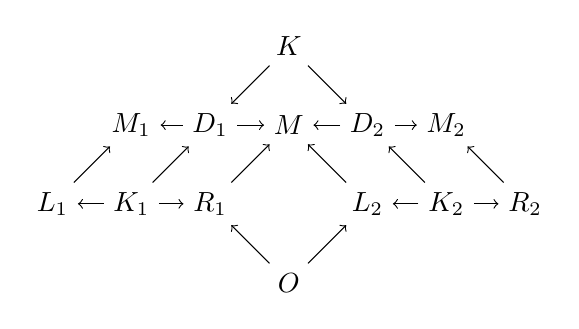
\begin{tikzpicture} %[scale=0.8]
  \node (o) at (0,-1) {\(O\)};
  \node (m) at (0,1) {\(M\)};
  \node (d2) at (1,1) {\(D_2\)};
  \node (m2) at (2,1) {\(M_2\)};
  \node (d1) at (-1,1) {\(D_1\)};
  \node (m1) at (-2,1) {\(M_1\)};
  \node (r1) at (-1,0) {\(R_1\)};
  \node (k1) at (-2,0) {\(K_1\)};
  \node (l1) at (-3,0) {\(L_1\)};
  \node (l2) at (1,0) {\(L_2\)};
  \node (k2) at (2,0) {\(K_2\)};
  \node (r2) at (3,0) {\(R_2\)};
  \node (k) at (0,2) {\(K\)};
  \draw [->] (o) -- (r1);
  \draw [->] (o) -- (l2);
  \draw [->] (r1) -- (m);
  \draw [->] (k1) -- (r1);
  \draw [->] (k1) -- (l1);
  \draw [->] (k1) -- (d1);
  \draw [->] (l1) -- (m1);
  \draw [->] (l2) -- (m);
  \draw [->] (k2) -- (r2);
  \draw [->] (k2) -- (l2);
  \draw [->] (k2) -- (d2);
  \draw [->] (r2) -- (m2);
  \draw [->] (d1) -- (m);
  \draw [->] (d1) -- (m1);
  \draw [->] (d2) -- (m);
  \draw [->] (d2) -- (m2);
  \draw [->] (k) -- (d1);
  \draw [->] (k) -- (d2);
\end{tikzpicture}
\]
\end{definition}

\autoref{def:ref_pos_infl} ressembles the definition of $E$-concurrent productions~\cite{AlgebraicGR}. However, $E$-concurrent productions combines two sequential dependent transitions into a single one, whereas~\autoref{def:ref_pos_infl} combines rules, linked by positive influence.

\begin{definition}[Refinement of two rewriting rules using positive and negative influence]
  \label{def:ref_pos_neg_infl}
  Let $r_1:L_1\remb K_1 \lemb R_1$ and $r_2:L_2\remb K_2 \lemb R_2$ be two rules.
  \begin{itemize}
  \item Let $s_1:R_1 \overset{o_1}{\lemb} O_1\overset{o_1'}{\remb} L_2$ and $s_2:R_1 \overset{o_2}{\lemb} O_2\overset{o_2'}{\remb} L_2$ be two cospans.
    \[
    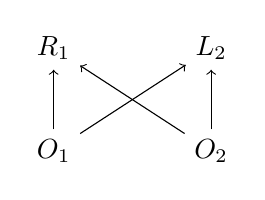
\begin{tikzpicture} %[scale=0.8]
      \node (o) at (1,-1.3) {\(O_2\)};
      \node (o2) at (-1,-1.3) {\(O_1\)};
      \node (r1) at (-1,0) {\(R_1\)};
      \node (l2) at (1,0) {\(L_2\)};
      \draw [->] (o) -- (r1);
      \draw [->] (o) -- (l2);
      \draw [->] (o2) -- (l2);
      \draw [->] (o2) -- (r1);
    \end{tikzpicture}
  \]
  Define $s_1\otimes s_2 = R_1\overset{o_3}{\lemb} O_3\overset{o_3'}{\remb} L_2$ as the cospan constructed as follows:
  \begin{itemize}
  \item let $O_3 = o_1(O_1)\cup o_2(O_2)$ be a subgraph of $R_1$ with $o_3:O_3\subseteq R_1$ the inclusion morphism;
  \item morphism $o_3':O_3\to L_2$ is defined as the union of the morphism $o_1^{-1}\circ o_2:o_1(O_1) \to L_2$ and $o_1'^{-1}\circ o_2':o_2(O_2) \to L_2$, where the morphisms $o_3$ and $o_3'$ are injective, and thus bijective on $\text{image}(O_1)$ and $\text{image}(O_2)$, respectively.
  \end{itemize}
  \item Let $s_1:R_1 \overset{o_1}{\lemb} O_1\overset{o_1'}{\remb} L_2$ be a span such that $r_1\redl{+}_{s_1} r_2$ and let $s_2:L_1 \overset{o_2}{\lemb} O_2\overset{o_2'}{\remb} L_2$ be a cospan such that $r_1\redl{-}_{s_2} r_2$ and $\neg(r_1\redl{-}_{O_2} r_2)$.
    Define $r_1\otimes_{s_1\otimes s_2} r_2 = r_1 \oplus_{s_3} r_2$, obtained as follows:
    \begin{itemize}
    \item if $l_1:K_1\emb L_1$ then $l_1^{-1}:\text{image}(l_1)\emb K_1$;
    \item the morphism $o_2:O_2\emb K_1$ is obtained by the composition of $f:O_2\emb L_1$ and $l_1^{-1}$. Moreover $f(O_2)\subseteq\text{image}(l_1)$ as otherwise, $r_1\redl{-}_{O_2} r_2$, which contradicts the hypothesis;
    \end{itemize}
  \[
  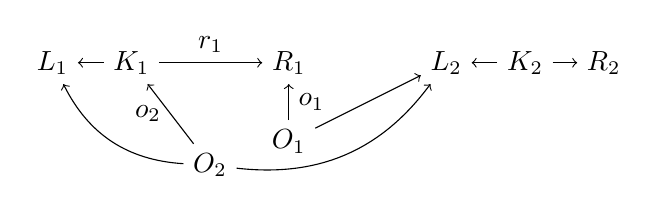
\begin{tikzpicture} %[scale=0.8]
  \node (o) at (-1,-1) {\(O_1\)};
  \node (o2) at (-2,-1.3) {\(O_2\)};
  \node (r1) at (-1,0) {\(R_1\)};
  \node (k1) at (-3,0) {\(K_1\)};
  \node (l1) at (-4,0) {\(L_1\)};
  \node (l2) at (1,0) {\(L_2\)};
  \node (k2) at (2,0) {\(K_2\)};
  \node (r2) at (3,0) {\(R_2\)};
  \draw [->] (o) -- node [right,midway] {\(o_1\)} (r1);
  \draw [->] (o) -- (l2);
  \draw [->] (k1) -- node [above,midway] {\(r_1\)} (r1);
  \draw [->] (k1) -- (l1);
  \draw [->] (k2) -- (r2);
  \draw [->] (k2) -- (l2);
  \draw [->] (o2) to [bend left] (l1);
  \draw [->] (o2) to [bend right] (l2);
  \draw [->] (o2) -- node [left,midway] {\(o_2\)} (k1);
  \end{tikzpicture}
  \]
  \end{itemize}
  %We write $e_1\otimes e_2 = \labl(e_1)\otimes_{O_1,O_2} \labl(e_2)$ to simplify notations.
\end{definition}
.

The spans are either positive or negative influences:
\begin{align*}
  \mathit{positive\_influences} = \{ \mathit{span}:R_i\remb O_i\lemb L \text{ where } e_i\redl{+}_{\mathit{span}} e, e_i\sqsubseteq e\} \\
  \mathit{negative\_influences} = \{ \mathit{span}:L_i\remb O_i\lemb L \text{ where } e\redl{-}_{\mathit{span}} e_i, e_i\sqsubseteq e\}
\end{align*}

Note that from~\autoref{def:linears}, for any events $e_i$,$e$ in an augmented poset, if $e_i\redl{+} e$ or $e\redl{-}e_i$ then $e_i\sqsubseteq e$.

\begin{definition}[Id graphs]
  We define an \emph{id graph} $G_I = (N,E)$ as a simple graphs $G = (V,E)$ where each node has associated an id unique in the graph: $n=(i,v)$ , where $v\in V$ and $i\in\nat$.
\end{definition}

Id graphs will help us keep track of the decorations.

\begin{remark}
\label{rm:simply}
  We make two simplifying assumptions. First, if an event uses an already introduced node than it appears in one of its decorations. All nodes in an event that are no part of any decorations are \emph{new} nodes that have \emph{fresh identifiers}, not used by any other node in the trace.

Secondly, we will assume that for any node there exists an event that introduces it. This assumption allows us to reason by induction on the linearisation of a poset.
\end{remark}

The following example shows how much the simplfying assumptions help.
\begin{example}
 Let us consider the poset of events $e_1,e_2,e_3,e_4$ with $e_3\dashv e_1$, $e_3\dashv e_2$ and all events $e_1,e_2,e_3$ causing event $e_4$. The rules are the following
 \begin{align*}
   r_1:A \Rightarrow A,B\qquad r_2:A \Rightarrow A,C \qquad r_3:A\Rightarrow D\qquad r_4:B,C,D\Rightarrow \varepsilon
 \end{align*}
 We can see that for such a poset we cannot construct the trace by induction on any linearisation. The constraint of node $A$ being the same node in both $e_1$ and $e_2$ only shows when event $e_3$ is considered.
\end{example}

We give the algorithm for $\mathsf{refine}$ below. It consists of first updating the graph $L$ of a production $p$ to account for all decorations in $\mathit{spans}$ (\autoref{eq:idprod1} to~\autoref{eq:idprod2}). Then a new transition $t$ is obtained from $p$ (\autoref{eq:newt}).
%Then the graphs in the trace are updated to account for the new added transition (\autoref{eq:newtrace}).
\begin{align}
  &\mathsf{refine}(\theta:M_1\Rightarrow M_2\cdots M_n,\mathtt{Ref},p:L\remb D\lemb R,\mathit{spans}) = \\
  \label{eq:idprod1}
  &\quad\mathit{id\_nodes} = \emptyset\\
  &\quad\text{for each }v\in L\\
  &\quad\qquad\text{if there exists }s:G\overset{g}{\remb}O\overset{o}{\lemb}L\text{ in }\mathit{spans}\text{ such that }
  o^{-1}(v)=v_o\in O\\
  &\quad\qquad\text{then }\mathit{id\_nodes} =\mathit{id\_nodes} \cup\{(v,\mathsf{id}(g(v_o))\}\\
  &\quad\qquad\text{else }\mathit{id\_nodes} =\mathit{id\_nodes} \cup\{(v,\mathit{fresh\_id})\}\\
  &\quad L_I = \mathsf{transform\_in_\_idgraph}(L,\mathit{id\_nodes})\\
  \label{eq:idprod2}
  &\quad p_I:L_I\remb D_I\lemb R_I = \mathsf{transform\_in_\_idproduction}(p,L_I)\\
  %&\quad M_n' = M_n\cup L_I \\
  \label{eq:newt}
  &\quad t = M_n\overset{L_I\lemb M_n,p}{\Rightarrow} M_{n+1}\\
  %\label{eq:newtrace}
  %&\quad \theta_2 = \mathsf{update\_trace}(M_1\Rightarrow M_2\cdots M_n, M_n\lemb M_n')\\
  &\quad \text{return }\theta;t
\end{align}

The trace $\theta:M_1\Rightarrow M_2\cdots M_n$ is obtained by induction on $s_1$, therefore $M_1,\cdots M_n$ are id graphs.

Let us first show that producing an id graph from $L$ in \autoref{eq:idprod1} to \autoref{eq:idprod2} is correct: there are no two decorations that disagree on the identifier of a node. The second part of the following lemma says that adding a new transition to the trace does not reintroduce node identifiers.

\begin{lemma}
  Let us suppose we have the following:
  \begin{itemize}
  \item two linear augmented posets $s_1$, $s_2$ such that $s_2=s_1\cup\{e\}$ and $e$ is maximal in $s_2$;
  \item two valid decorations for the two posets $s_1^{\star}$ and $s_2^{\star}$ with $s_2^{\star}\subseteq s_1^{\star}$;
  \item a trace $\theta:M_1\Rightarrow M_2\cdots M_n$ such that $\mathsf{decoration\_of\_trace}(\theta)=(s_1)^{\star}$ and such that $M_1,\cdots M_n$ are id graphs;
  \end{itemize}
  \begin{enumerate}
  \item For two decorations of $e$ in $s_2^{\star}$, $\mathit{span}_1$ and $\mathit{span}_2$ such that either
    \begin{enumerate}
    \item $R_1 \overset{g_1}{\remb} O_1 \overset{o_1}{\lemb} L \overset{o_2}{\remb} O_2\overset{g_2}{\lemb} R_2$ or
    \item $L_1 \overset{g_1}{\remb} O_1 \overset{o_1}{\lemb} L \overset{o_2}{\remb} O_2\overset{g_2}{\lemb} L_2$ or
    \item $L_1 \overset{g_1}{\remb} O_1 \overset{o_1}{\lemb} L \overset{o_2}{\remb} O_2\overset{g_2}{\lemb} R_2$.
    \end{enumerate}
    we have that for all $n\in L$ such that $o_1^{-1}(n) = n_1\in O$ and $o_2^{-1}(n) = n_2\in O$, $\text{id}(g_1(n_1)) = \text{id}(g_2(n_2))$.
  \item Let $L_I$ be the id graph constructed as in \autoref{eq:idprod1} to~\autoref{eq:idprod2}. Then $L_I\subseteq M_n$.
\end{enumerate}
\end{lemma}
\begin{proof}
  \begin{enumerate}
  \item
  \begin{enumerate}
  \item It follows that there exists $e_1,e_2\in s_2^{\star}$ such that $e_1\redl{+}_{\mathit{span}_1} e$ and $e_2\redl{+}_{\mathit{span}_2} e$ and that the constraint on decorating positive meets in~\autoref{def:constraints_poset} is not satisfied. Contradiction with the hypothesis that $s_2^{\star}$ is a valid decoration.
  \item Thanks to our symplifying assumption~\autoref{rm:simply} there exists an event $e_3$ which introduces node $n_1$. It follows then $e_3\redl{+}_{\mathit{span}_3} e_1$ where node $n_1$ is in the decoration $\mathit{span}_3$. Either $e_3\redl{+}_{\mathit{span}_3'} e_2$ with $n_2$ in the decoration $\mathit{span}_3'$ in which case, by induction we have that $\text{id}(n_1) = \text{id}(n_2)$, or $\neg(e_3\redl{+}_{\mathit{span}_3'} e_2)$. This contradicts the constraint on decorating forks of negative influence in~\autoref{def:constraints_poset}.
  \item It follows that there exists $e_1,e_2\in s_2^{\star}$ such that $e_2\redl{+}_{\mathit{span}_2} e$ and $e\redl{-}_{\mathit{span}_2} e_1$. But then there exists a span ${\mathit{span}_3}$ such that $e_2\redl{+}_{\mathit{span}_3} e_1$ and the constraint on decorating positive forks in~\autoref{def:constraints_poset} is again not satisfied.
  \end{enumerate}
  \item Suppose that there exists $n\in L_I$ and $n\notin M_n$. From the symplifying assumption~\autoref{rm:simply} there exists an event $e_1$ which introduces node $n$. But $n\notin M_n$, implies that there exists an event $e_2$ which "consumes" $n$, i.e. $e_1\redl{+}_n e_2$ and $e_2\redl{-}_n e$. %we cannot use this last part $e_2\redl{-}_n e$ because we haven't yet proved that the concretisation of s2 doesn't introduce extra decorations.
From $e_1\redl{+}_n e_2$ and $e_1\redl{+}_n e$ we have that the constraint on decorating positive forks in~\autoref{def:constraints_poset} is not satisfied.
  \end{enumerate}
\end{proof}

%A corollary for the second part of the lemma above is that the $\mathsf{refine}$ function does not create extra decorations, i.e. $\mathsf{decoration\_of\_trace}(\theta_2)=(s_2)^{\star}$. This is one part in the correction theorem below.

\begin{theorem}
  Let $s_1$ be a linear augmented poset, let $\theta_1$ be a trace and $\mathtt{Ref}_1$ a refinement function on $\theta_1$ such that for any events $e_1,e_2\in s_1$
  \begin{align}
    \label{eq1}
    e_1\prec e_2 \iff& \mathtt{Ref}(e_1) \prec_{\theta}\mathtt{Ref}(e_2)\\
    \label{eq2}
    e_1\Dashv e_2 \iff& \mathtt{Ref}(e_1) \dashv_{\theta}\mathtt{Ref}(e_2)
  \end{align}
  Let $s_2$ be a linear augmented poset such that $s_2=s_1\cup\{e\}$ and $e$ is maximal in $s_2$.
  For any $\theta_2$ and $\mathtt{Ref}_2$ obtained by $\mathsf{concretise}(s_2,s_1,\{(\theta_1,\mathtt{Ref}_1)\})$ the conditions~\autoref{eq1}, \autoref{eq2} hold.
\end{theorem}
\begin{proof}
  Let $s_1^{\star}$ be a decoration of $s_1$ such that $\mathsf{decoration\_of\_trace}(\theta_1)=(s_1)^{\star}$.
  First we note that we can translate conditions~\autoref{eq1}, \autoref{eq2} on decorations:
  \begin{align*}
    e_1\prec e_2 \iff&e_1\redl{+}_s e_2 \iff \mathtt{Ref}(e_1) \prec_{\theta}^{s}\mathtt{Ref}(e_2)\\
    e_1\Dashv e_2 \iff&e_1\redl{-}_s e_2 \iff \mathtt{Ref}(e_1) \dashv_{\theta}^{s}\mathtt{Ref}(e_2)
  \end{align*}
\end{proof}
